% answers.tex —— 2005 年·普通高等学校招生考试·湖北卷·文科 · 参考答案与详细解析片段
% 由 tools/generate_projects.py 依来源总账自 2005/2005_数学真题_湖北文科_试题.md + 2005/2005_数学真题_湖北文科_解析正文.md + 2005/2005_数学真题_湖北文科_答案要点.md 生成，勿手改（改源 MD 后重跑）

\begin{answer}
\gksolhead{1}{}

\textbf{题目}：

设 $P$、$Q$ 为两个非空实数集合，定义集合 $P + Q = \{a + b \mid a \in P, b \in Q\}$，若 $P = \{0, 2, 5\}, Q = \{1, 2, 6\}$，则 $P + Q$ 中元素的个数是\mbox{（　　）}

\begin{gkopts}(4)
\task A．9
\task B．8
\task C．7
\task D．6
\end{gkopts}

\Needspace{4\baselineskip}
\textbf{解析}

根据题意，集合 $P + Q$ 中的元素由 $a \in P$ 与 $b \in Q$ 的所有可能和构成：
\begin{itemize}
\item 取 $a = 0$ 时：$0 + 1 = 1$，$0 + 2 = 2$，$0 + 6 = 6$；
\item 取 $a = 2$ 时：$2 + 1 = 3$，$2 + 2 = 4$，$2 + 6 = 8$；
\item 取 $a = 5$ 时：$5 + 1 = 6$（已存在），$5 + 2 = 7$，$5 + 6 = 11$．
\end{itemize}

\Needspace{5\baselineskip}
综合去重后得到集合：
\nopagebreak[4]
\[
P + Q = \{1, 2, 3, 4, 6, 7, 8, 11\}.
\]
元素个数共有 8 个．

故选 B．

\gkanswer{答案：B}

\end{answer}
\begin{answer}
\gksolhead{2}{}

\textbf{题目}：

对任意实数 $a, b, c$，给出下列命题：

① “$a = b$”是“$ac = bc$”充要条件；

② “$a + 5$ 是无理数”是“$a$ 是无理数”的充要条件；

③ “$a > b$”是“$a^2 > b^2$”的充分条件；

④ “$a < 5$”是“$a < 3$”的必要条件．

其中真命题的个数是\mbox{（　　）}

\begin{gkopts}(4)
\task A．1
\task B．2
\task C．3
\task D．4
\end{gkopts}

\Needspace{4\baselineskip}
\textbf{解析}

逐一分析各命题的真假：
\begin{itemize}
\item 对于 ①：若 $c = 0$，由 $ac = bc$ 不能推得 $a = b$，故“$a = b$”是“$ac = bc$”的充分不必要条件，① 为假命题；
\item 对于 ②：若 $a$ 为无理数，假设 $a + 5 = r \in \mathbf{Q}$，则 $a = r - 5 \in \mathbf{Q}$，矛盾，故 $a + 5$ 必为无理数；反之，若 $a + 5$ 为无理数，假设 $a = r \in \mathbf{Q}$，则 $a + 5 = r + 5 \in \mathbf{Q}$，亦矛盾，故 $a$ 必为无理数．因此“$a + 5$ 是无理数”是“$a$ 是无理数”的充要条件，② 为真命题；
\item 对于 ③：取 $a = 1, b = -2$，满足 $a > b$，但 $a^2 = 1 < b^2 = 4$，充分性不成立，③ 为假命题；
\item 对于 ④：若 $a < 3$，则显然满足 $a < 5$，即 $(-\infty, 3) \subset (-\infty, 5)$，因此“$a < 5$”是“$a < 3$”的必要条件，④ 为真命题．
\end{itemize}

综上，真命题共有 ②、④ 两个．

故选 B．

\gkanswer{答案：B}

\end{answer}
\begin{answer}
\gksolhead{3}{}

\textbf{题目}：

已知向量 $\vec{a} = (-2, 2), \vec{b} = (5, k)$．若 $|\vec{a} + \vec{b}|$ 不超过 5，则 $k$ 的取值范围是\mbox{（　　）}

\begin{gkopts}(4)
\task A．$[-4, 6]$
\task B．$[-6, 4]$
\task C．$[-6, 2]$
\task D．$[-2, 6]$
\end{gkopts}

\Needspace{4\baselineskip}
\textbf{解析}

\Needspace{5\baselineskip}
由向量坐标线性加法运算得：
\nopagebreak[4]
\[
\vec{a} + \vec{b} = (-2 + 5, 2 + k) = (3, 2 + k).
\]
\Needspace{5\baselineskip}
其模长为：
\nopagebreak[4]
\[
|\vec{a} + \vec{b}| = \sqrt{3^2 + (2 + k)^2} = \sqrt{9 + (k + 2)^2}.
\]
\Needspace{5\baselineskip}
由题意 $|\vec{a} + \vec{b}| \leqslant 5$，两边平方得：
\nopagebreak[4]
\[
9 + (k + 2)^2 \leqslant 25 \iff (k + 2)^2 \leqslant 16 \iff -4 \leqslant k + 2 \leqslant 4.
\]
\Needspace{5\baselineskip}
解得：
\nopagebreak[4]
\[
-6 \leqslant k \leqslant 2.
\]

故选 C．

\gkanswer{答案：C}

\end{answer}
\begin{answer}
\gksolhead{4}{}

\textbf{题目}：

函数 $y = \mathrm{e}^{|\ln x|} - |x - 1|$ 的图象大致是\mbox{（　　）}
\nopagebreak[4]
\begin{center}% 2005 年湖北卷文科第 4 题选项图：函数 y = e^{|\ln x|} - |x-1| 的图象 4 个选项
\begin{tikzpicture}[>=stealth,scale=0.9,line cap=round]
  % 统一设置单图尺寸与间距
  % (A)
  \begin{scope}
    \draw[->] (-0.8,0) -- (2.6,0) node[below] {$x$};
    \draw[->] (0,-0.8) -- (0,2.6) node[left] {$y$};
    \node[below left] at (0,0) {$O$};
    \draw (1,0.08) -- (1,-0.08) node[below] {$1$};
    \draw (0.08,1) -- (-0.08,1) node[left] {$1$};
    % (A): y = 1 for x in (0, 2.2], (0, 1) is empty circle
    \draw[thick] (0.06,1) -- (2.2,1);
    \draw[fill=white] (0,1) circle (1.5pt);
    \node at (-0.6,-1.1) {(A)};
  \end{scope}

  % (B)
  \begin{scope}[xshift=5.8cm]
    \draw[->] (-0.8,0) -- (2.6,0) node[below] {$x$};
    \draw[->] (0,-0.8) -- (0,2.6) node[left] {$y$};
    \node[below left] at (0,0) {$O$};
    \draw (1,0.08) -- (1,-0.08) node[below left] {$1$};
    \draw (0.08,1) -- (-0.08,1) node[left] {$1$};
    % (B): x in [1, 2.2] is y=1; x in (0.3, 1) is increasing curve to (1, 0.4)
    \draw[thick] (1,1) -- (2.2,1);
    \draw[dashed] (1,0) -- (1,1);
    \draw[dashed] (0,1) -- (1,1);
    \draw[dashed] (1,0) -- (1,0.4);
    \draw[thick,domain=0.35:0.96,samples=30] plot (\x,{0.4*sqrt(\x) + 0.8*(\x-1)});
    \draw[fill=white] (1,0.4) circle (1.5pt);
    \node at (-0.6,-1.1) {(B)};
  \end{scope}

  % (C)
  \begin{scope}[yshift=-4.8cm]
    \draw[->] (-0.8,0) -- (2.6,0) node[below] {$x$};
    \draw[->] (0,-0.8) -- (0,2.6) node[left] {$y$};
    \node[below left] at (0,0) {$O$};
    \draw (1,0.08) -- (1,-0.08) node[below] {$1$};
    \draw (0.08,1) -- (-0.08,1) node[left] {$1$};
    % (C): x in (0.35, 1) decreasing curve to (1, 1), x in [1, 2.0] increasing line
    \draw[dashed] (1,0) -- (1,1);
    \draw[dashed] (0,1) -- (1,1);
    \draw[thick,domain=0.35:1,samples=30] plot (\x,{\x + 1/\x - 1});
    \draw[thick] (1,1) -- (2.0,2.0);
    \node at (-0.6,-1.1) {(C)};
  \end{scope}

  % (D) 正确选项
  \begin{scope}[xshift=5.8cm,yshift=-4.8cm]
    \draw[->] (-0.8,0) -- (2.6,0) node[below] {$x$};
    \draw[->] (0,-0.8) -- (0,2.6) node[left] {$y$};
    \node[below left] at (0,0) {$O$};
    \draw (1,0.08) -- (1,-0.08) node[below] {$1$};
    \draw (0.08,1) -- (-0.08,1) node[left] {$1$};
    % (D): x in (0.35, 1) decreasing convex curve y = x + 1/x - 1 to (1, 1), x in [1, 2.2] horizontal line y=1
    \draw[dashed] (1,0) -- (1,1);
    \draw[dashed] (0,1) -- (1,1);
    \draw[thick,domain=0.35:1,samples=40] plot (\x,{\x + 1/\x - 1});
    \draw[thick] (1,1) -- (2.2,1);
    \node at (-0.6,-1.1) {(D)};
  \end{scope}
\end{tikzpicture}
\end{center}
\nopagebreak[4]
\begin{gkopts}(1)
\task A．在 $x > 0$ 上恒等于 1 的水平射线（不含点 $(0, 1)$）
\task B．在 $(0, 1)$ 上递增、在 $[1, +\infty)$ 上恒等于 1 的图象
\task C．在 $(0, 1)$ 上递减、在 $[1, +\infty)$ 上斜向上递增的折线
\task D．在 $(0, 1)$ 上为下凸递减曲线、在 $[1, +\infty)$ 上为水平射线 $y = 1$ 的图象
\end{gkopts}

\Needspace{4\baselineskip}
\textbf{解析}

对自变量 $x > 0$ 进行分段讨论：
1. 当 $0 < x < 1$ 时，$\ln x < 0$，从而 $|\ln x| = -\ln x$，$\mathrm{e}^{|\ln x|} = \mathrm{e}^{-\ln x} = \dfrac{1}{x}$．
   此时 $|x - 1| = -(x - 1) = 1 - x$．
\Needspace{5\baselineskip}
   因此：
\nopagebreak[4]
\[
y = \frac{1}{x} - (1 - x) = x + \frac{1}{x} - 1.
\]
   在 $(0, 1)$ 上，$y' = 1 - \dfrac{1}{x^2} = \dfrac{x^2 - 1}{x^2} < 0$，函数单调递减；
   且 $y'' = \dfrac{2}{x^3} > 0$，函数图象下凸；
   当 $x \to 1^-$ 时，$y \to 1 + 1 - 1 = 1$．
2. 当 $x \geqslant 1$ 时，$\ln x \geqslant 0$，从而 $|\ln x| = \ln x$，$\mathrm{e}^{|\ln x|} = \mathrm{e}^{\ln x} = x$．
   此时 $|x - 1| = x - 1$．
\Needspace{5\baselineskip}
   因此：
\nopagebreak[4]
\[
y = x - (x - 1) = 1.
\]
   函数恒为常数 1，图象为一条从 $(1, 1)$ 开始水平向右的射线．

由于 $\lim_{x \to 1^-} y = 1 = y(1)$，函数在 $x = 1$ 处连续．
对照各选项图象，选项 (D) 正确展示了在 $(0, 1)$ 上单调下凸递减连接至 $(1, 1)$，随后在 $[1, +\infty)$ 上保持水平射线 $y = 1$ 的形态．

故选 D．

\gkanswer{答案：D}

\end{answer}
\begin{answer}
\gksolhead{5}{}

\textbf{题目}：

木星的体积约是地球体积的 $240\sqrt{30}$ 倍，则它的表面积约是地球表面积的\mbox{（　　）}

\begin{gkopts}(2)
\task A．60 倍
\task B．$60\sqrt{30}$ 倍
\task C．120 倍
\task D．$120\sqrt{30}$ 倍
\end{gkopts}

\Needspace{4\baselineskip}
\textbf{解析}

将木星与地球均视为球体，设木星半径为 $R_1$，地球半径为 $R_2$．
\Needspace{5\baselineskip}
由球体体积公式 $V = \dfrac{4}{3}\pi R^3$ 可知，体积之比等于半径比的立方：
\nopagebreak[4]
\[
\frac{V_1}{V_2} = \left(\frac{R_1}{R_2}\right)^3 = 240\sqrt{30}.
\]
\Needspace{5\baselineskip}
因为：
\nopagebreak[4]
\[
(240\sqrt{30})^2 = 240^2 \times 30 = 57600 \times 30 = 1728000 = 120^3,
\]
所以 $240\sqrt{30} = 120^{3/2} = (120^{1/2})^3$．
\Needspace{5\baselineskip}
由此解得相似比（半径比）：
\nopagebreak[4]
\[
\frac{R_1}{R_2} = \sqrt{120}.
\]
\Needspace{5\baselineskip}
根据球体表面积公式 $S = 4\pi R^2$，表面积比等于半径比的平方：
\nopagebreak[4]
\[
\frac{S_1}{S_2} = \left(\frac{R_1}{R_2}\right)^2 = (\sqrt{120})^2 = 120.
\]
即木星的表面积约是地球表面积的 120 倍．

故选 C．

\gkanswer{答案：C}

\end{answer}
\begin{answer}
\gksolhead{6}{}

\textbf{题目}：

双曲线 $\dfrac{x^2}{m} - \dfrac{y^2}{n} = 1$ ($mn \neq 0$) 离心率为 2，有一个焦点与抛物线 $y^2 = 4x$ 的焦点重合，则 $mn$ 的值为\mbox{（　　）}

\begin{gkopts}(4)
\task A．$\dfrac{3}{16}$
\task B．$\dfrac{3}{8}$
\task C．$\dfrac{16}{3}$
\task D．$\dfrac{8}{3}$
\end{gkopts}

\Needspace{4\baselineskip}
\textbf{解析}

抛物线 $y^2 = 4x$ 的标准形式为 $y^2 = 2px$（其中 $p = 2$），其焦点坐标为 $(1, 0)$．
因为双曲线 $\dfrac{x^2}{m} - \dfrac{y^2}{n} = 1$ ($mn \neq 0$) 的焦点与抛物线焦点重合，
所以双曲线的焦点在 $x$ 轴上，右焦点为 $(1, 0)$，即半焦距 $c = 1$．
\Needspace{5\baselineskip}
由双曲线的离心率 $e = \dfrac{c}{a} = 2$，解得：
\nopagebreak[4]
\[
a = \frac{c}{e} = \frac{1}{2}.
\]
\Needspace{5\baselineskip}
从而：
\nopagebreak[4]
\[
m = a^2 = \left(\frac{1}{2}\right)^2 = \frac{1}{4}.
\]
\Needspace{5\baselineskip}
又由双曲线中 $c^2 = a^2 + b^2 = m + n$，得：
\nopagebreak[4]
\[
n = c^2 - m = 1 - \frac{1}{4} = \frac{3}{4}.
\]
\Needspace{5\baselineskip}
因此：
\nopagebreak[4]
\[
mn = \frac{1}{4} \times \frac{3}{4} = \frac{3}{16}.
\]

故选 A．

\gkanswer{答案：A}

\end{answer}
\begin{answer}
\gksolhead{7}{}

\textbf{题目}：

在 $y = 2^x, y = \log_2 x, y = x^2, y = \cos 2x$ 这四个函数中，当 $0 < x_1 < x_2 < 1$ 时，使 $f\left(\dfrac{x_1 + x_2}{2}\right) > \dfrac{f(x_1) + f(x_2)}{2}$ 恒成立的函数的个数是\mbox{（　　）}

\begin{gkopts}(4)
\task A．0
\task B．1
\task C．2
\task D．3
\end{gkopts}

\Needspace{4\baselineskip}
\textbf{解析}

条件 $f\left(\dfrac{x_1 + x_2}{2}\right) > \dfrac{f(x_1) + f(x_2)}{2}$（对任意 $0 < x_1 < x_2 < 1$ 恒成立）是函数 $f(x)$ 在区间 $(0, 1)$ 上为严格上凸函数（二阶导数 $f''(x) < 0$）的充分必要条件．
逐一检验四个函数在 $(0, 1)$ 上的凸凹性：
1. 对 $f(x) = 2^x$：导数 $f'(x) = 2^x \ln 2$，$f''(x) = 2^x (\ln 2)^2 > 0$，函数为下凸函数，不满足条件；
2. 对 $f(x) = \log_2 x$：导数 $f'(x) = \dfrac{1}{x \ln 2}$，$f''(x) = -\dfrac{1}{x^2 \ln 2} < 0$，函数为严格上凸函数，满足条件；
3. 对 $f(x) = x^2$：导数 $f'(x) = 2x$，$f''(x) = 2 > 0$，函数为下凸函数，不满足条件；
4. 对 $f(x) = \cos 2x$：当 $x \in (0, 1)$ 时，$2x \in (0, 2)$．二阶导数为 $f''(x) = -4\cos 2x$．
   当 $2x \in \left(0, \dfrac{\pi}{2}\right)$（即 $x \in \left(0, \dfrac{\pi}{4}\right)$）时，$\cos 2x > 0 \implies f''(x) < 0$；
   但当 $2x \in \left(\dfrac{\pi}{2}, 2\right)$（即 $x \in \left(\dfrac{\pi}{4}, 1\right)$）时，$\cos 2x < 0 \implies f''(x) > 0$（函数转为下凸）．
   因此在整个区间 $(0, 1)$ 上不等式不恒成立．

综上，满足条件的函数只有 $y = \log_2 x$ 一个．

故选 B．

\gkanswer{答案：B}

\end{answer}
\begin{answer}
\gksolhead{8}{}

\textbf{题目}：

已知 $a, b, c$ 是直线，$\beta$ 是平面，给出下列命题：

① 若 $a \perp b, b \perp c$，则 $a \parallel c$；

② 若 $a \parallel b, b \perp c$，则 $a \perp c$；

③ 若 $a \parallel \beta, b \subset \beta$，则 $a \parallel b$；

④ 若 $a$ 与 $b$ 异面，且 $a \parallel \beta$，则 $b, \beta$ 相交；

⑤ 若 $a$ 与 $b$ 异面，则至多有一条直线与 $a, b$ 都垂直．

其中真命题的个数是\mbox{（　　）}

\begin{gkopts}(4)
\task A．1
\task B．2
\task C．3
\task D．4
\end{gkopts}

\Needspace{4\baselineskip}
\textbf{解析}

逐一分析空间线面关系的命题真假：
\begin{itemize}
\item 对于 ①：在空间中垂直于同一条直线的两条直线，可以平行、相交或异面（如正方体中从同一顶点出发的三条相互垂直的棱），故 ① 为假命题；
\item 对于 ②：根据空间线面垂直性质，两条平行直线中的一条垂直于第三条直线，则另一条也必垂直于该直线，故 ② 为真命题；
\item 对于 ③：直线与平面平行，则该直线与平面内的直线既可能平行，也可能异面，故 ③ 为假命题；
\item 对于 ④：若 $a$ 与 $b$ 异面且 $a \parallel \beta$，$b$ 与平面 $\beta$ 可以平行（例如 $a, b$ 分别位于两个平行平面内且不平行，平面 $\beta$ 平行于这两个平面），不一定相交，故 ④ 为假命题；
\item 对于 ⑤：两条异面直线的公垂线只有一条（公垂线段所在直线），但与 $a, b$ 都垂直的直线有无数条（凡是以两异面直线方向向量的外积方向为方向向量的所有平行直线，都同时垂直于 $a$ 和 $b$），故 ⑤ 称“至多有一条”为假命题．
\end{itemize}

综上，真命题只有 ② 一个．

故选 A．

\gkanswer{答案：A}

\end{answer}
\begin{answer}
\gksolhead{9}{}

\textbf{题目}：

把一同排 6 张座位编号为 1, 2, 3, 4, 5, 6 的电影票全部分给 4 个人，每人至少分 1 张，至多分 2 张，且拿 2 张票的人这两张票具有连续的编号，那么不同的分法种数是\mbox{（　　）}

\begin{gkopts}(4)
\task A．168
\task B．96
\task C．72
\task D．144
\end{gkopts}

\Needspace{4\baselineskip}
\textbf{解析}

将 6 张连续编号的电影票分给 4 个人，每人至少 1 张、至多 2 张：
因为 $1 \leqslant x_i \leqslant 2$ 且 $\sum_{i=1}^4 x_i = 6$，所以只能有两人各分得 2 张、两人各分得 1 张（组容量为 $2, 2, 1, 1$）．
根据题意，分得 2 张票的两个人，手里的票都必须具有连续的编号．
这相当于把连续序列 $1, 2, 3, 4, 5, 6$ 分解为两个长度为 2 的连续块 $X_1, X_2$ 和两个长度为 1 的单元 $Y_1, Y_2$：
\Needspace{5\baselineskip}
在 4 个分块的位置序列中，选择 2 个位置放置长度为 2 的连续块，划分方案数为：
\nopagebreak[4]
\[
\mathrm{C}_4^2 = \frac{4 \times 3}{2} = 6 \text{ \text{种}}.
\]
这 6 种连续组划分具体为：

\begin{itemize}
\item ① $\{1, 2\}, \{3, 4\}, \{5\}, \{6\}$；
\item ② $\{1, 2\}, \{3\}, \{4, 5\}, \{6\}$；
\item ③ $\{1, 2\}, \{3\}, \{4\}, \{5, 6\}$；
\item ④ $\{1\}, \{2, 3\}, \{4, 5\}, \{6\}$；
\item ⑤ $\{1\}, \{2, 3\}, \{4\}, \{5, 6\}$；
\item ⑥ $\{1\}, \{2\}, \{3, 4\}, \{5, 6\}$．
\end{itemize}

\Needspace{5\baselineskip}
每种划分得到 4 个互不相同的包裹，将其分配给 4 个不同的人，全排列数为：
\nopagebreak[4]
\[
\mathrm{A}_4^4 = 4! = 24 \text{ \text{种}}.
\]
\Needspace{5\baselineskip}
由乘法原理，不同的分法总数为：
\nopagebreak[4]
\[
6 \times 24 = 144 \text{ \text{种}}.
\]

故选 D．

\gkanswer{答案：D}

\end{answer}
\begin{answer}
\gksolhead{10}{}

\textbf{题目}：

若 $\sin\alpha + \cos\alpha = \tan\alpha$ $\left(0 < \alpha < \dfrac{\pi}{2}\right)$，则 $\alpha \in$\mbox{（　　）}

\begin{gkopts}(2)
\task A．$\left(0, \dfrac{\pi}{6}\right)$
\task B．$\left(\dfrac{\pi}{6}, \dfrac{\pi}{4}\right)$
\task C．$\left(\dfrac{\pi}{4}, \dfrac{\pi}{3}\right)$
\task D．$\left(\dfrac{\pi}{3}, \dfrac{\pi}{2}\right)$
\end{gkopts}

\Needspace{4\baselineskip}
\textbf{解析}

设函数 $g(\alpha) = \sin\alpha + \cos\alpha - \tan\alpha$，在开区间 $\left(0, \dfrac{\pi}{2}\right)$ 内考察：
\begin{itemize}
\item 当 $\alpha = \dfrac{\pi}{4}$ 时：
\end{itemize}
\nopagebreak[4]
\[
\sin\frac{\pi}{4} + \cos\frac{\pi}{4} = \frac{\sqrt{2}}{2} + \frac{\sqrt{2}}{2} = \sqrt{2}, \quad \tan\frac{\pi}{4} = 1.
\]
  由于 $\sqrt{2} > 1$，所以 $g\left(\dfrac{\pi}{4}\right) = \sqrt{2} - 1 > 0$．
\begin{itemize}
\item 当 $\alpha = \dfrac{\pi}{3}$ 时：
\end{itemize}
\nopagebreak[4]
\[
\sin\frac{\pi}{3} + \cos\frac{\pi}{3} = \frac{\sqrt{3}}{2} + \frac{1}{2} = \frac{\sqrt{3} + 1}{2} \approx \frac{2.732}{2} = 1.366, \quad \tan\frac{\pi}{3} = \sqrt{3} \approx 1.732.
\]
  由于 $1.366 < 1.732$，所以 $g\left(\dfrac{\pi}{3}\right) < 0$．

因为 $g(\alpha)$ 在闭区间 $\left[\dfrac{\pi}{4}, \dfrac{\pi}{3}\right]$ 上连续，且端点值异号（$g(\pi/4) > 0, g(\pi/3) < 0$），
根据连续函数的零点存在性定理，方程必在区间 $\left(\dfrac{\pi}{4}, \dfrac{\pi}{3}\right)$ 内存在解．

故选 C．

\gkanswer{答案：C}

\end{answer}
\begin{answer}
\gksolhead{11}{}

\textbf{题目}：

在函数 $y = x^3 - 8x$ 的图象上，其切线的倾斜角小于 $\dfrac{\pi}{4}$ 的点中，坐标为整数的点的个数是\mbox{（　　）}

\begin{gkopts}(4)
\task A．3
\task B．2
\task C．1
\task D．0
\end{gkopts}

\Needspace{4\baselineskip}
\textbf{解析}

\Needspace{5\baselineskip}
设曲线上点的横坐标为 $x$．切线的斜率为导数值：
\nopagebreak[4]
\[
k = y' = 3x^2 - 8.
\]
平面直角坐标系中，直线的倾斜角 $\theta$ 取值范围为 $[0, \pi)$．
\Needspace{5\baselineskip}
切线的倾斜角小于 $\dfrac{\pi}{4}$，即：
\nopagebreak[4]
\[
0 \leqslant \theta < \frac{\pi}{4}.
\]
\Needspace{5\baselineskip}
因为正切函数在 $\left[0, \dfrac{\pi}{4}\right)$ 上单调递增，所以其斜率 $k = \tan\theta$ 必须满足：
\nopagebreak[4]
\[
0 \leqslant k < \tan\frac{\pi}{4} = 1.
\]
（若 $k < 0$，其倾斜角 $\theta \in \left(\dfrac{\pi}{2}, \pi\right) > \dfrac{\pi}{4}$，不符合题意）．
\Needspace{5\baselineskip}
代入导数表达式得：
\nopagebreak[4]
\[
0 \leqslant 3x^2 - 8 < 1 \iff 8 \leqslant 3x^2 < 9 \iff \frac{8}{3} \leqslant x^2 < 3.
\]
若曲线上点 $(x, y)$ 为整数点，则 $x$ 必为整数（由 $y = x^3 - 8x$ 可知此时 $y$ 亦为整数）．
但由于 $x \in \mathbf{Z}$ 时，$x^2$ 的可能取值为 $0, 1, 4, 9, \dots$，不存在任何整数使其平方落在半开区间 $\left[\dfrac{8}{3}, 3\right)$ 内．
因此，满足题意的整数点个数为 0．

故选 D．

\gkanswer{答案：D}

\end{answer}
\begin{answer}
\gksolhead{12}{}

\textbf{题目}：

某初级中学有学生 270 人，其中一年级 108 人，二、三年级各 81 人，现要利用抽样方法抽取 10 人参加某项调查，考虑选用简单随机抽样、分层抽样和系统抽样三种方案，使用简单随机抽样和分层抽样时，将学生按一、二、三年级依次统一编号为 $1, 2, \dots, 270$；使用系统抽样时，将学生统一随机编号 $1, 2, \dots, 270$，并将整个编号依次分为 10 段．如果抽得号码有下列四种情况：

① $7, 34, 61, 88, 115, 142, 169, 196, 223, 250$；

② $5, 9, 100, 107, 111, 121, 180, 195, 200, 265$；

③ $11, 38, 65, 92, 119, 146, 173, 200, 227, 254$；

④ $30, 57, 84, 111, 138, 165, 192, 219, 246, 270$；

关于上述样本的下列结论中，正确的是\mbox{（　　）}

\begin{gkopts}(2)
\task A．②、③都不能为系统抽样
\task B．②、④都不能为分层抽样
\task C．①、④都可能为系统抽样
\task D．①、③都可能为分层抽样
\end{gkopts}

\Needspace{4\baselineskip}
\textbf{解析}

1. \textbf{系统抽样分析}：
   总体容量 $N = 270$，抽取样本容量 $n = 10$，分段间隔为 $k = \dfrac{270}{10} = 27$．
   系统抽样要求在第 1 段 $[1, 27]$ 中随机抽取起始号 $r$，后续各段抽取的编号为 $r + 27m$ ($m = 0, 1, \dots, 9$)，且公差严格为 27．
\begin{itemize}
\item 对 ①：编号 $7, 34, 61, \dots, 250$ 中，首项 $7 \in [1, 27]$，公差为 27，末项 $250 \in [244, 270]$，完全符合系统抽样；
\item 对 ③：编号 $11, 38, 65, \dots, 254$ 中，首项 $11 \in [1, 27]$，公差为 27，末项 $254 \in [244, 270]$，完全符合系统抽样；
\item 对 ④：首项为 30，超出第一段 $[1, 27]$，不符合系统抽样规范；
\item 对 ②：公差不恒定，不是系统抽样．
\end{itemize}
2. \textbf{分层抽样分析}：
   三个年级人数分别为一年级 108 人（编号 $1 \sim 108$）、二年级 81 人（编号 $109 \sim 189$）、三年级 81 人（编号 $190 \sim 270$）．
   抽样比为 $\dfrac{10}{270} = \dfrac{1}{27}$，各层应抽样本量为：
\begin{itemize}
\item 一年级：$108 \times \dfrac{1}{27} = 4$ 人；
\item 二年级：$81 \times \dfrac{1}{27} = 3$ 人；
\item 三年级：$81 \times \dfrac{1}{27} = 3$ 人．
\end{itemize}
   检查各编号在三个年级区间的分布：
\begin{itemize}
\item 样本 ①：$[1, 108]$ 内有 4 个（$7, 34, 61, 88$）；$[109, 189]$ 内有 3 个（$115, 142, 169$）；$[190, 270]$ 内有 3 个（$196, 223, 250$），满足 $4 : 3 : 3$ 配额，可能为分层抽样；
\item 样本 ③：$[1, 108]$ 内有 4 个（$11, 38, 65, 92$）；$[109, 189]$ 内有 3 个（$119, 146, 173$）；$[190, 270]$ 内有 3 个（$200, 227, 254$），满足 $4 : 3 : 3$ 配额，可能为分层抽样；
\item 样本 ④：$[1, 108]$ 内仅有 3 个（$30, 57, 84$），$[190, 270]$ 内有 4 个，不符合配额要求，不能为分层抽样．
\end{itemize}

综上，结论“①、③都可能为分层抽样”正确．

故选 D．

\gkanswer{答案：D}

\end{answer}
\begin{answer}
\gksolhead{13}{}

\textbf{题目}：

函数 $f(x) = \dfrac{\sqrt{x - 2}}{x - 3}\lg\sqrt{4 - x}$ 的定义域是 $\underline{\qquad\qquad}$．

\Needspace{4\baselineskip}
\textbf{解析}

要使函数有意义，自变量 $x$ 须满足以下三个条件：
1. 偶次根号下被开方数非负：$x - 2 \geqslant 0 \implies x \geqslant 2$；
2. 分式分母不为零：$x - 3 \neq 0 \implies x \neq 3$；
3. 对数真数大于零：$\sqrt{4 - x} > 0 \implies 4 - x > 0 \implies x < 4$．

\Needspace{5\baselineskip}
联立上述不等式组：
\nopagebreak[4]
\[
\begin{cases}
x \geqslant 2, \\
x \neq 3, \\
x < 4.
\end{cases}
\]
解得函数的定义域为 $[2, 3) \cup (3, 4)$．

\gkanswer{答案：$[2, 3) \cup (3, 4)$（或 $\{x \mid 2 \leqslant x < 4 \text{ \text{且} } x \neq 3\}$）。}

\end{answer}
\begin{answer}
\gksolhead{14}{}

\textbf{题目}：

$\left(x^3 - \dfrac{2}{x}\right)^4 + \left(x + \dfrac{1}{x}\right)^8$ 的展开式中整理后的常数项等于 $\underline{\qquad\qquad}$．

\Needspace{4\baselineskip}
\textbf{解析}

分别求出两项二项展开式中的常数项：
1. 对于 $\left(x^3 - \dfrac{2}{x}\right)^4$：
\Needspace{5\baselineskip}
   展开式的通项为：
\nopagebreak[4]
\[
T_{r+1} = \mathrm{C}_4^r (x^3)^{4-r} \left(-\frac{2}{x}\right)^r = \mathrm{C}_4^r (-2)^r x^{12 - 4r}.
\]
   令 $12 - 4r = 0$，解得 $r = 3$．
\Needspace{5\baselineskip}
   常数项为：
\nopagebreak[4]
\[
\mathrm{C}_4^3 (-2)^3 = 4 \times (-8) = -32.
\]
2. 对于 $\left(x + \dfrac{1}{x}\right)^8$：
\Needspace{5\baselineskip}
   展开式的通项为：
\nopagebreak[4]
\[
T_{k+1} = \mathrm{C}_8^k x^{8-k} \left(\frac{1}{x}\right)^k = \mathrm{C}_8^k x^{8-2k}.
\]
   令 $8 - 2k = 0$，解得 $k = 4$．
\Needspace{5\baselineskip}
   常数项为：
\nopagebreak[4]
\[
\mathrm{C}_8^4 = \frac{8 \times 7 \times 6 \times 5}{4 \times 3 \times 2 \times 1} = 70.
\]

\Needspace{5\baselineskip}
两部分常数项相加得：
\nopagebreak[4]
\[
-32 + 70 = 38.
\]

\gkanswer{答案：$38$。}

\end{answer}
\begin{answer}
\gksolhead{15}{}

\textbf{题目}：

函数 $y = |\sin x|\cos x - 1$ 的最小正周期与最大值的和为 $\underline{\qquad\qquad}$．

\Needspace{4\baselineskip}
\textbf{解析}

设 $g(x) = |\sin x|\cos x$．
1. \textbf{最小正周期}：
   因为 $|\sin(x + \pi)| = |-\sin x| = |\sin x|$，而 $\cos(x + \pi) = -\cos x$，
   所以 $g(x + \pi) = -g(x)$，进而 $g(x + 2\pi) = g(x)$．
   当 $x \in (0, \pi)$ 时，$\sin x > 0 \implies g(x) = \dfrac{1}{2}\sin 2x$；当 $x \in (\pi, 2\pi)$ 时，$\sin x < 0 \implies g(x) = -\dfrac{1}{2}\sin 2x$．
   方程 $g(x) = \dfrac{1}{2}$ 在区间 $[0, 2\pi)$ 内仅有唯一解 $x = \dfrac{\pi}{4}$，故 $g(x)$ 的最小正周期为 $2\pi$．
2. \textbf{最大值}：
\Needspace{5\baselineskip}
   由绝对值不等式与基本不等式：
\nopagebreak[4]
\[
|\sin x|\cos x \leqslant |\sin x| |\cos x| \leqslant \frac{\sin^2 x + \cos^2 x}{2} = \frac{1}{2}.
\]
   当 $x = \dfrac{\pi}{4}$ 时，$g\left(\dfrac{\pi}{4}\right) = \dfrac{\sqrt{2}}{2} \times \dfrac{\sqrt{2}}{2} = \dfrac{1}{2}$ 取得最大值．
\Needspace{5\baselineskip}
   因此原函数的最大值为：
\nopagebreak[4]
\[
y_{\max} = \frac{1}{2} - 1 = -\frac{1}{2}.
\]

\Needspace{5\baselineskip}
最小正周期与最大值的和为：
\nopagebreak[4]
\[
2\pi + \left(-\frac{1}{2}\right) = 2\pi - \frac{1}{2}.
\]

\gkanswer{答案：$2\pi - \dfrac{1}{2}$。}

\end{answer}
\begin{answer}
\gksolhead{16}{}

\textbf{题目}：

某实验室需购某种化工原料 106 千克，现在市场上该原料有两种包装，一种是每袋 35 千克，价格为 140 元；另一种是每袋 24 千克，价格为 120 元．在满足需要的条件下，最少要花费 $\underline{\qquad\qquad}$ 元．

\Needspace{4\baselineskip}
\textbf{解析}

设购买每袋 35 千克的原料 $x$ 袋，每袋 24 千克的原料 $y$ 袋，其中 $x, y \in \mathbf{N}$．
\Needspace{5\baselineskip}
根据题意需满足总量约束：
\nopagebreak[4]
\[
35x + 24y \geqslant 106.
\]
目标是使总花费 $C = 140x + 120y$ 最小．
比较两包装的单位单价：
\begin{itemize}
\item 35 千克包装：$\dfrac{140}{35} = 4$ 元/千克；
\item 24 千克包装：$\dfrac{120}{24} = 5$ 元/千克．
\end{itemize}
应优先使用单价更低的 35 千克包装：
\begin{itemize}
\item 若 $x = 0$：$24y \geqslant 106 \implies y \geqslant 5$，花费 $120 \times 5 = 600$ 元；
\item 若 $x = 1$：$24y \geqslant 106 - 35 = 71 \implies y \geqslant 3$，总重 $35 + 72 = 107$ 千克，花费 $140 \times 1 + 120 \times 3 = 140 + 360 = 500$ 元；
\item 若 $x = 2$：$24y \geqslant 106 - 70 = 36 \implies y \geqslant 2$，总重 $70 + 48 = 118$ 千克，花费 $140 \times 2 + 120 \times 2 = 280 + 240 = 520$ 元；
\item 若 $x = 3$：$24y \geqslant 106 - 105 = 1 \implies y \geqslant 1$，总重 $105 + 24 = 129$ 千克，花费 $140 \times 3 + 120 \times 1 = 420 + 120 = 540$ 元；
\item 若 $x = 4$：$35 \times 4 = 140 \geqslant 106$（取 $y = 0$），花费 $140 \times 4 = 560$ 元．
\end{itemize}

比较可知，当 $x = 1, y = 3$ 时花费最少，最少花费为 500 元．

\gkanswer{答案：$500$。}

\end{answer}
\begin{answer}
\gksolhead{17}{}

\textbf{题目}：

（本小题满分 12 分）

已知向量 $\vec{a} = (x^2, x + 1), \vec{b} = (1 - x, t)$，若函数 $f(x) = \vec{a} \cdot \vec{b}$ 在区间 $(-1, 1)$ 上是增函数，求 $t$ 的取值范围．

\Needspace{4\baselineskip}
\textbf{解析}

\Needspace{5\baselineskip}
由向量数量积的坐标公式：
\nopagebreak[4]
\[
f(x) = \vec{a} \cdot \vec{b} = x^2(1 - x) + t(x + 1) = -x^3 + x^2 + tx + t.
\]
\Needspace{5\baselineskip}
对其求导得：
\nopagebreak[4]
\[
f'(x) = -3x^2 + 2x + t.
\]
\Needspace{5\baselineskip}
若函数 $f(x)$ 在区间 $(-1, 1)$ 上是增函数，则导数在该区间上必须恒非负：
\nopagebreak[4]
\[
f'(x) = -3x^2 + 2x + t \geqslant 0 \quad (\forall x \in (-1, 1)).
\]
\Needspace{5\baselineskip}
分离参数得：
\nopagebreak[4]
\[
t \geqslant 3x^2 - 2x \quad (\forall x \in (-1, 1)).
\]
设 $g(x) = 3x^2 - 2x = 3\left(x - \dfrac{1}{3}\right)^2 - \dfrac{1}{3}$．
函数 $g(x)$ 是对称轴为 $x = \dfrac{1}{3}$、开口向上的二次函数．
\Needspace{5\baselineskip}
在闭区间 $[-1, 1]$ 上端点值分别为：
\nopagebreak[4]
\[
g(-1) = 3(-1)^2 - 2(-1) = 5, \quad g(1) = 3(1)^2 - 2(1) = 1.
\]
所以在开区间 $(-1, 1)$ 上，$g(x) < 5$，其上确界为 $\sup_{x \in (-1, 1)} g(x) = 5$．
\Needspace{5\baselineskip}
要使不等式 $t \geqslant g(x)$ 对任意 $x \in (-1, 1)$ 恒成立，必须且只需：
\nopagebreak[4]
\[
t \geqslant 5.
\]
（当 $t = 5$ 时，$f'(x) = -3x^2 + 2x + 5 = (5 - 3x)(x + 1)$，在区间 $(-1, 1)$ 内恒有 $f'(x) > 0$，函数确实严格单调递增）．

故 $t$ 的取值范围是 $[5, +\infty)$．

\gkanswer{答案：$[5, +\infty)$。}

\end{answer}
\begin{answer}
\gksolhead{18}{}

\textbf{题目}：

（本小题满分 12 分）

在 $\triangle ABC$ 中，已知 $\tan B = \sqrt{3}, \cos C = \dfrac{1}{3}, AC = 3\sqrt{6}$，求 $\triangle ABC$ 的面积．

\Needspace{4\baselineskip}
\textbf{解析}

\Needspace{5\baselineskip}
因为 $\tan B = \sqrt{3}$ 且 $B \in (0, \pi)$，所以：
\nopagebreak[4]
\[
B = \frac{\pi}{3}, \quad \sin B = \frac{\sqrt{3}}{2}, \quad \cos B = \frac{1}{2}.
\]
\Needspace{5\baselineskip}
因为 $\cos C = \dfrac{1}{3}$ 且 $C \in (0, \pi)$，所以：
\nopagebreak[4]
\[
\sin C = \sqrt{1 - \cos^2 C} = \sqrt{1 - \left(\frac{1}{3}\right)^2} = \frac{2\sqrt{2}}{3}.
\]
\Needspace{5\baselineskip}
根据两角和的正弦公式：
\nopagebreak[4]
\[
\sin A = \sin(\pi - (B + C)) = \sin(B + C) = \sin B \cos C + \cos B \sin C.
\]
\Needspace{5\baselineskip}
代入已知数值：
\nopagebreak[4]
\[
\sin A = \frac{\sqrt{3}}{2} \times \frac{1}{3} + \frac{1}{2} \times \frac{2\sqrt{2}}{3} = \frac{\sqrt{3} + 2\sqrt{2}}{6}.
\]
\Needspace{5\baselineskip}
在 $\triangle ABC$ 中，已知边 $b = AC = 3\sqrt{6}$，由正弦定理：
\nopagebreak[4]
\[
\frac{c}{\sin C} = \frac{b}{\sin B} \implies c = AB = \frac{b \sin C}{\sin B}.
\]
\Needspace{5\baselineskip}
代入数值：
\nopagebreak[4]
\[
c = \frac{3\sqrt{6} \times \dfrac{2\sqrt{2}}{3}}{\dfrac{\sqrt{3}}{2}} = \frac{2\sqrt{12}}{\dfrac{\sqrt{3}}{2}} = \frac{4\sqrt{3}}{\dfrac{\sqrt{3}}{2}} = 8.
\]
\Needspace{5\baselineskip}
利用三角形面积公式：
\nopagebreak[4]
\[
\begin{aligned}
S_{\triangle ABC} &= \frac{1}{2} b c \sin A = \frac{1}{2} \times 3\sqrt{6} \times 8 \times \frac{\sqrt{3} + 2\sqrt{2}}{6} \\
&= 2\sqrt{6} (\sqrt{3} + 2\sqrt{2}) = 2\sqrt{18} + 4\sqrt{12} = 6\sqrt{2} + 8\sqrt{3}.
\end{aligned}
\]

故 $\triangle ABC$ 的面积为 $6\sqrt{2} + 8\sqrt{3}$．

\gkanswer{答案：$6\sqrt{2} + 8\sqrt{3}$。}

\end{answer}
\begin{answer}
\gksolhead{19}{}

\textbf{题目}：

（本小题满分 12 分）

设数列 $\{a_n\}$ 的前 $n$ 项和为 $S_n = 2n^2$，$\{b_n\}$ 为等比数列，且 $a_1 = b_1, b_2(a_2 - a_1) = b_1$．

(1) 求数列 $\{a_n\}$ 和 $\{b_n\}$ 的通项公式；

(2) 设 $c_n = \dfrac{a_n}{b_n}$，求数列 $\{c_n\}$ 的前 $n$ 项和 $T_n$．

\Needspace{4\baselineskip}
\textbf{解析}

\textbf{(1)}

当 $n = 1$ 时，$a_1 = S_1 = 2 \times 1^2 = 2$．
\Needspace{5\baselineskip}
当 $n \geqslant 2$ 时：
\nopagebreak[4]
\[
a_n = S_n - S_{n-1} = 2n^2 - 2(n - 1)^2 = 2(2n - 1) = 4n - 2.
\]
当 $n = 1$ 时，$4(1) - 2 = 2 = a_1$ 同样满足．
\Needspace{5\baselineskip}
所以数列 $\{a_n\}$ 的通项公式为：
\nopagebreak[4]
\[
a_n = 4n - 2 \quad (n \in \mathbf{N}^*).
\]
由此可知 $a_2 = 4(2) - 2 = 6$，$a_2 - a_1 = 6 - 2 = 4$．
因为 $a_1 = b_1$，所以 $b_1 = 2$．
设等比数列 $\{b_n\}$ 的公比为 $q$，则 $b_2 = b_1 q = 2q$．
\Needspace{5\baselineskip}
代入条件 $b_2(a_2 - a_1) = b_1$ 得：
\nopagebreak[4]
\[
(2q) \times 4 = 2 \implies 8q = 2 \implies q = \frac{1}{4}.
\]
\Needspace{5\baselineskip}
所以等比数列 $\{b_n\}$ 的通项公式为：
\nopagebreak[4]
\[
b_n = 2 \times \left(\frac{1}{4}\right)^{n-1} = \frac{1}{2^{2n-3}} \quad (n \in \mathbf{N}^*).
\]

\textbf{(2)}

\Needspace{5\baselineskip}
由 $c_n = \dfrac{a_n}{b_n}$ 得：
\nopagebreak[4]
\[
c_n = \frac{4n - 2}{2 \times (1/4)^{n-1}} = (2n - 1) \cdot 4^{n-1}.
\]
\Needspace{5\baselineskip}
前 $n$ 项和为：
\nopagebreak[4]
\[
T_n = 1 \cdot 1 + 3 \cdot 4^1 + 5 \cdot 4^2 + \dots + (2n - 1) \cdot 4^{n-1}.
\]
\Needspace{5\baselineskip}
两边同乘以 4 得：
\nopagebreak[4]
\[
4T_n = 1 \cdot 4^1 + 3 \cdot 4^2 + \dots + (2n - 3) \cdot 4^{n-1} + (2n - 1) \cdot 4^n.
\]
\Needspace{5\baselineskip}
两式相减得：
\nopagebreak[4]
\[
-3T_n = 1 + 2(4^1 + 4^2 + \dots + 4^{n-1}) - (2n - 1) \cdot 4^n.
\]
\Needspace{5\baselineskip}
利用等比数列求和公式：
\nopagebreak[4]
\[
4^1 + 4^2 + \dots + 4^{n-1} = \frac{4(4^{n-1} - 1)}{4 - 1} = \frac{4^n - 4}{3}.
\]
\Needspace{5\baselineskip}
代入得：
\nopagebreak[4]
\[
-3T_n = 1 + \frac{2(4^n - 4)}{3} - (2n - 1) \cdot 4^n = \frac{3 + 2 \cdot 4^n - 8 - 3(2n - 1) \cdot 4^n}{3} = \frac{-5 + (5 - 6n) \cdot 4^n}{3}.
\]
\Needspace{5\baselineskip}
两边同除以 $-3$：
\nopagebreak[4]
\[
T_n = \frac{(6n - 5) \cdot 4^n + 5}{9}.
\]

\gkanswer{答案（1）：$a_n = 4n - 2$；$b_n = 2 \times \left(\dfrac{1}{4}\right)^{n-1} = \dfrac{1}{2^{2n-3}}$。}

\gkanswer{答案（2）：$T_n = \dfrac{(6n - 5) \cdot 4^n + 5}{9}$。}

\end{answer}
\begin{answer}
\gksolhead{20}{}

\textbf{题目}：

（本小题满分 12 分）

如图所示的多面体是由底面为 $ABCD$ 的长方体被截面 $AEC_1F$ 所截而得到的，其中 $AB = 4, BC = 2, CC_1 = 3, BE = 1$．
\nopagebreak[4]
\begin{center}% 2005 年湖北卷文科第 20 题配图：长方体被截面 AEC_1F 截得的多面体
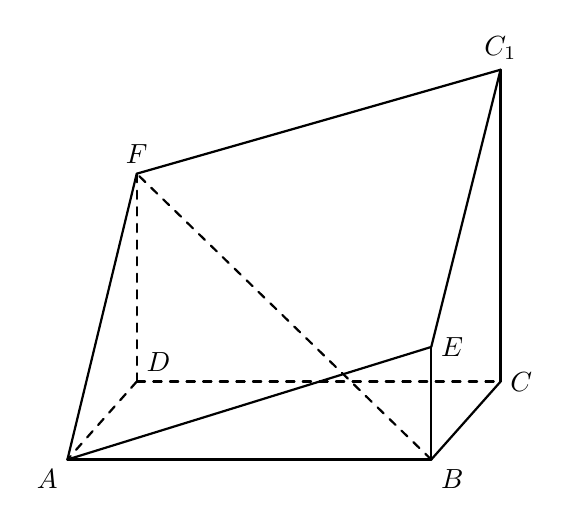
\begin{tikzpicture}[>=stealth,scale=1.1,line cap=round,line join=round]
  % 顶点坐标设定
  \coordinate (D) at (0,0);
  \coordinate (C) at (4.2,0);
  \coordinate (A) at (-0.8,-0.9);
  \coordinate (B) at (3.4,-0.9);
  \coordinate (C1) at (4.2,3.6);
  \coordinate (E) at (3.4,0.4);
  \coordinate (F) at (0,2.4);

  % 虚线不可见棱及内部辅助线
  \draw[dashed,thick] (D) -- (A);
  \draw[dashed,thick] (D) -- (C);
  \draw[dashed,thick] (D) -- (F);
  \draw[dashed,thick] (B) -- (F);

  % 实线可见棱及截面边界
  \draw[thick] (A) -- (B);
  \draw[thick] (B) -- (C);
  \draw[thick] (C) -- (C1);
  \draw[thick] (B) -- (E);
  \draw[thick] (A) -- (E);
  \draw[thick] (E) -- (C1);
  \draw[thick] (C1) -- (F);
  \draw[thick] (F) -- (A);

  % 顶点标签
  \node[below left] at (A) {$A$};
  \node[below right] at (B) {$B$};
  \node[right] at (C) {$C$};
  \node[above right] at (D) {$D$};
  \node[above] at (C1) {$C_1$};
  \node[right] at (E) {$E$};
  \node[above] at (F) {$F$};
\end{tikzpicture}
\end{center}
\nopagebreak[4]
(1) 求 $BF$ 的长；

(2) 求点 $C$ 到平面 $AEC_1F$ 的距离．

\Needspace{4\baselineskip}
\textbf{解析}

\textbf{(1)}

设长方体底面边长 $AB = 4, BC = 2$，垂直侧棱 $CC_1 = 3$．
以点 $D$ 为坐标原点，建立空间直角坐标系：
\begin{itemize}
\item $DA$ 为 $x$ 轴正方向：$D(0, 0, 0), A(2, 0, 0)$；
\item $DC$ 为 $y$ 轴正方向：$C(0, 4, 0)$；
\item $DD_1$ 为 $z$ 轴正方向．
\end{itemize}
则 $B(2, 4, 0)$，$C_1(0, 4, 3)$．
因为点 $E$ 在侧棱 $BB_1$ 上，且 $BE = 1$，所以 $E(2, 4, 1)$．
设点 $F$ 在侧棱 $DD_1$ 上的坐标为 $F(0, 0, h)$（其中 $h = DF$）．
因为截面 $AEC_1F$ 为一平面，所以四边形 $AEC_1F$ 的四个顶点共面．
\Needspace{5\baselineskip}
又因为长方体的相对侧面平行（面 $ABB_1A_1 \parallel$ 面 $DCC_1D_1$），平面 $AEC_1F$ 与这两相对平面的交线必互相平行：
\nopagebreak[4]
\[
AF \parallel EC_1.
\]
从而向量 $\vec{AF}$ 与 $\vec{EC_1}$ 平行且方向一致．
\Needspace{5\baselineskip}
计算向量坐标：
\nopagebreak[4]
\[
\vec{EC_1} = (0 - 2, 4 - 4, 3 - 1) = (-2, 0, 2),
\]
\nopagebreak[4]
\[
\vec{AF} = (0 - 2, 0 - 0, h - 0) = (-2, 0, h).
\]
\Needspace{5\baselineskip}
由 $\vec{AF} = \vec{EC_1}$ 立即得到：
\nopagebreak[4]
\[
h = 2, \quad \text{\text{即} } DF = 2.
\]
在直角三角形 $\triangle BDF$ 中，因为 $FD \perp$ 底面 $ABCD$，所以 $FD \perp BD$．
\Needspace{5\baselineskip}
底面对角线长为：
\nopagebreak[4]
\[
BD = \sqrt{AB^2 + AD^2} = \sqrt{4^2 + 2^2} = \sqrt{20}.
\]
\Needspace{5\baselineskip}
因此：
\nopagebreak[4]
\[
BF = \sqrt{BD^2 + DF^2} = \sqrt{20 + 2^2} = \sqrt{24} = 2\sqrt{6}.
\]

\textbf{(2)}

\Needspace{5\baselineskip}
由 (1) 可知点 $F(0, 0, 2)$，向量：
\nopagebreak[4]
\[
\vec{AF} = (-2, 0, 2), \quad \vec{AE} = (2 - 2, 4 - 0, 1 - 0) = (0, 4, 1).
\]
\Needspace{5\baselineskip}
设平面 $AEC_1F$ 的法向量为 $\vec{n} = (x, y, z)$，则：
\nopagebreak[4]
\[
\begin{cases}
\vec{n} \cdot \vec{AF} = -2x + 2z = 0 \implies z = x, \\
\vec{n} \cdot \vec{AE} = 4y + z = 0 \implies y = -\dfrac{z}{4} = -\dfrac{x}{4}.
\end{cases}
\]
\Needspace{5\baselineskip}
取 $x = 4$，则 $z = 4, y = -1$，得法向量：
\nopagebreak[4]
\[
\vec{n} = (4, -1, 4).
\]
\Needspace{5\baselineskip}
其模长为：
\nopagebreak[4]
\[
|\vec{n}| = \sqrt{4^2 + (-1)^2 + 4^2} = \sqrt{16 + 1 + 16} = \sqrt{33}.
\]
因为点 $C_1(0, 4, 3)$ 位于平面 $AEC_1F$ 内，取向量 $\vec{CC_1} = (0, 0, 3)$，
\Needspace{5\baselineskip}
则点 $C$ 到平面 $AEC_1F$ 的距离为：
\nopagebreak[4]
\[
d = \frac{|\vec{CC_1} \cdot \vec{n}|}{|\vec{n}|} = \frac{|0 \times 4 + 0 \times (-1) + 3 \times 4|}{\sqrt{33}} = \frac{12}{\sqrt{33}} = \frac{4\sqrt{33}}{11}.
\]

\gkanswer{答案（1）：$BF = 2\sqrt{6}$。}

\gkanswer{答案（2）：$\dfrac{4\sqrt{33}}{11}$。}

\end{answer}
\begin{answer}
\gksolhead{21}{}

\textbf{题目}：

（本小题满分 12 分）

某会议室用 5 盏灯照明，每盏灯各使用灯泡一只，且型号相同．假定每盏灯能否正常照明只与灯泡的寿命有关，该型号的灯泡寿命为 1 年以上的概率为 $p_1$，寿命为 2 年以上的概率为 $p_2$．从使用之日起每满 1 年进行一次灯泡更换工作，只更换已坏的灯泡，平时不换．

(1) 在第一次灯泡更换工作中，求不需要换灯泡的概率和更换 2 只灯泡的概率；

(2) 在第二次灯泡更换工作中，对其中的某一盏灯来说，求该盏灯需要更换灯泡的概率；

(3) 当 $p_1 = 0.8, p_2 = 0.3$ 时，求在第二次灯泡更换工作，至少需要更换 4 只灯泡的概率．（结果保留两个有效数字）

\Needspace{4\baselineskip}
\textbf{解析}

\textbf{(1)}

设每只新灯泡的寿命为 $X$．已知 $P(X > 1) = p_1$，所以在 1 年内损坏的概率为 $1 - p_1$．
在第 1 年末的第一次更换工作中，5 盏灯各使用 1 只使用满 1 年的灯泡，各灯互不影响：
\begin{itemize}
\item 不需要更换灯泡（即 5 只灯泡均未坏）的概率为：
\end{itemize}
\nopagebreak[4]
\[
P_0 = p_1^5.
\]
\begin{itemize}
\item 恰好需要更换 2 只灯泡（即 2 只损坏、3 只完好）的概率为：
\end{itemize}
\nopagebreak[4]
\[
P_2 = \mathrm{C}_5^2 (1 - p_1)^2 p_1^3 = 10(1 - p_1)^2 p_1^3.
\]

\textbf{(2)}

考察第 2 年末的第二次更换工作中某一特定盏灯的状况：
该灯在第 1 年末有两种互斥情形：
\begin{itemize}
\item 情形一：第 1 年末该灯泡未坏（概率为 $p_1$），未曾更换．到第 2 年末时该灯泡已连续使用 2 年，它在第 2 年内坏掉（即寿命超过 1 年但不超过 2 年）的概率为：
\end{itemize}
\nopagebreak[4]
\[
P(1 < X \leqslant 2) = P(X > 1) - P(X > 2) = p_1 - p_2.
\]
\begin{itemize}
\item 情形二：第 1 年末该灯泡已坏（概率为 $1 - p_1$），更换为新灯泡．换上的新灯泡在接下来的第 2 年（即使用 1 年内）坏掉的概率为 $1 - p_1$．由独立性，这一情形下在第 2 年末再次损坏的概率为：
\end{itemize}
\nopagebreak[4]
\[
(1 - p_1) \times (1 - p_1) = (1 - p_1)^2.
\]
\Needspace{5\baselineskip}
由全概率公式，该盏灯在第二次更换工作中需要更换灯泡的概率为：
\nopagebreak[4]
\[
p = (p_1 - p_2) + (1 - p_1)^2 = 1 - p_1 - p_2 + p_1^2.
\]

\textbf{(3)}

\Needspace{5\baselineskip}
当 $p_1 = 0.8, p_2 = 0.3$ 时，代入 (2) 中公式计算单盏灯在第 2 年末更换的概率：
\nopagebreak[4]
\[
p = (0.8 - 0.3) + (1 - 0.8)^2 = 0.5 + 0.04 = 0.54.
\]
在第二次更换工作中，需要更换的灯泡总数 $\xi \sim B(5, 0.54)$．
至少需要更换 4 只灯泡即 $\xi = 4$ 或 $\xi = 5$：
\begin{itemize}
\item $P(\xi = 4) = \mathrm{C}_5^4 p^4 (1 - p) = 5 \times 0.54^4 \times (1 - 0.54) = 5 \times 0.54^4 \times 0.46 = 2.3 \times 0.54^4$；
\item $P(\xi = 5) = p^5 = 0.54^5 = 0.54 \times 0.54^4$．
\end{itemize}
\Needspace{5\baselineskip}
因此：
\nopagebreak[4]
\[
P(\xi \geqslant 4) = (2.3 + 0.54) \times 0.54^4 = 2.84 \times 0.54^4.
\]
\Needspace{5\baselineskip}
计算数值：
\nopagebreak[4]
\[
0.54^2 = 0.2916, \quad 0.54^4 = 0.08503056,
\]
\nopagebreak[4]
\[
P(\xi \geqslant 4) = 2.84 \times 0.08503056 = 0.24148679\dots
\]
保留两个有效数字，所求概率约为 $0.24$．

\gkanswer{答案（1）：不需要换灯泡的概率为 $p_1^5$；更换 2 只灯泡的概率为 $10(1 - p_1)^2 p_1^3$。}

\gkanswer{答案（2）：$(1 - p_1)^2 + p_1 - p_2$。}

\gkanswer{答案（3）：$0.24$。}

\end{answer}
\begin{answer}
\gksolhead{22}{}

\textbf{题目}：

（本小题满分 14 分）

设 $A, B$ 是椭圆 $3x^2 + y^2 = \lambda$ 上的两点，点 $N(1, 3)$ 是线段 $AB$ 的中点，线段 $AB$ 的垂直平分线与椭圆相交于 $C, D$ 两点．

(1) 确定 $\lambda$ 的取值范围，并求直线 $AB$ 的方程；

(2) 试判断是否存在这样的 $\lambda$，使得 $A, B, C, D$ 四点在同一个圆上？并说明理由．

\Needspace{4\baselineskip}
\textbf{解析}

\textbf{(1)}

\Needspace{5\baselineskip}
设 $A(x_1, y_1), B(x_2, y_2)$，点 $N(1, 3)$ 为线段 $AB$ 的中点，则：
\nopagebreak[4]
\[
x_1 + x_2 = 2, \quad y_1 + y_2 = 6.
\]
\Needspace{5\baselineskip}
由于点 $A, B$ 均在椭圆 $3x^2 + y^2 = \lambda$ 上，代入坐标得：
\nopagebreak[4]
\[
3x_1^2 + y_1^2 = \lambda, \quad 3x_2^2 + y_2^2 = \lambda.
\]
\Needspace{5\baselineskip}
两式相减（点差法）：
\nopagebreak[4]
\[
3(x_1 - x_2)(x_1 + x_2) + (y_1 - y_2)(y_1 + y_2) = 0.
\]
若 $x_1 = x_2$，则直线 $AB$ 垂直于 $x$ 轴，其中点纵坐标应为 0，与中点纵坐标为 3 矛盾，故 $x_1 \neq x_2$．
\Needspace{5\baselineskip}
两边同除以 $x_1 - x_2$：
\nopagebreak[4]
\[
3(x_1 + x_2) + k_{AB}(y_1 + y_2) = 0 \implies 3(2) + 6 k_{AB} = 0 \implies k_{AB} = -1.
\]
\Needspace{5\baselineskip}
因此直线 $AB$ 经过点 $N(1, 3)$ 且斜率为 $-1$，其方程为：
\nopagebreak[4]
\[
y - 3 = -(x - 1) \implies x + y - 4 = 0.
\]
\Needspace{5\baselineskip}
将 $y = 4 - x$ 代入椭圆方程 $3x^2 + y^2 = \lambda$：
\nopagebreak[4]
\[
3x^2 + (4 - x)^2 = \lambda \implies 4x^2 - 8x + 16 - \lambda = 0.
\]
\Needspace{5\baselineskip}
因为直线 $AB$ 与椭圆交于两相异点，其判别式必须大于零：
\nopagebreak[4]
\[
\Delta_1 = (-8)^2 - 4 \times 4(16 - \lambda) = 16(\lambda - 12) > 0 \implies \lambda > 12.
\]
又因为线段 $AB$ 的垂直平分线 $CD$ 与 $AB$ 垂直，其斜率为 $k_{CD} = -\dfrac{1}{k_{AB}} = 1$，且经过中点 $N(1, 3)$，
\Needspace{5\baselineskip}
所以直线 $CD$ 的方程为：
\nopagebreak[4]
\[
y - 3 = x - 1 \implies y = x + 2.
\]
\Needspace{5\baselineskip}
将 $y = x + 2$ 代入椭圆方程得：
\nopagebreak[4]
\[
3x^2 + (x + 2)^2 = \lambda \implies 4x^2 + 4x + 4 - \lambda = 0.
\]
判别式 $\Delta_2 = 16 - 16(4 - \lambda) = 16(\lambda - 3) > 0 \implies \lambda > 3$．
由于 $\lambda > 12$ 蕴含 $\lambda > 3$，故 $\lambda$ 的取值范围为 $(12, +\infty)$．

\textbf{(2)}

存在，事实上对于任意 $\lambda \in (12, +\infty)$，四点 $A, B, C, D$ 恒在同一个圆上．理由如下：
因为直线 $CD$ 垂直平分线段 $AB$，相交于点 $N(1, 3)$，两弦 $AB \perp CD$．
\Needspace{5\baselineskip}
根据相交弦定理及其逆定理，若四点 $A, B, C, D$ 共圆，充分必要条件为：
\nopagebreak[4]
\[
|NA| \cdot |NB| = |NC| \cdot |ND|.
\]
下面分别计算两乘积：
1. 因为 $N$ 为 $AB$ 中点，所以 $|NA| = |NB| = \dfrac{|AB|}{2}$．
   由二次方程 $4x^2 - 8x + 16 - \lambda = 0$，根与系数关系为 $x_1 + x_2 = 2, x_1 x_2 = \dfrac{16 - \lambda}{4}$．
   从而 $(x_1 - x_2)^2 = (x_1 + x_2)^2 - 4x_1 x_2 = 4 - (16 - \lambda) = \lambda - 12$．
\Needspace{5\baselineskip}
   由于 $k_{AB} = -1$，弦长平方为：
\nopagebreak[4]
\[
|AB|^2 = (1 + k^2)(x_1 - x_2)^2 = 2(\lambda - 12).
\]
\Needspace{5\baselineskip}
   因此：
\nopagebreak[4]
\[
|NA| \cdot |NB| = \frac{|AB|^2}{4} = \frac{\lambda - 12}{2}.
\]
2. 设点 $C(x_3, y_3), D(x_4, y_4)$，其中 $x_3, x_4$ 为二次方程 $4x^2 + 4x + 4 - \lambda = 0$ 的两根．
   由根与系数关系：$x_3 + x_4 = -1$，$x_3 x_4 = \dfrac{4 - \lambda}{4}$．
\Needspace{5\baselineskip}
   点 $N$ 的横坐标为 1，故：
\nopagebreak[4]
\[
(x_3 - 1)(x_4 - 1) = x_3 x_4 - (x_3 + x_4) + 1 = \frac{4 - \lambda}{4} - (-1) + 1 = 3 - \frac{\lambda}{4} = -\frac{\lambda - 12}{4}.
\]
   当 $\lambda > 12$ 时，$(x_3 - 1)(x_4 - 1) < 0$，说明点 $N$ 严格位于线段 $CD$ 内部．
\Needspace{5\baselineskip}
   因为直线 $CD$ 斜率为 1，所以：
\nopagebreak[4]
\[
|NC| = \sqrt{1 + 1^2} |x_3 - 1| = \sqrt{2}|x_3 - 1|, \quad |ND| = \sqrt{2}|x_4 - 1|.
\]
\Needspace{5\baselineskip}
   从而：
\nopagebreak[4]
\[
|NC| \cdot |ND| = 2 |(x_3 - 1)(x_4 - 1)| = 2 \times \frac{\lambda - 12}{4} = \frac{\lambda - 12}{2}.
\]

\Needspace{5\baselineskip}
由此证得，对任意 $\lambda > 12$，恒有：
\nopagebreak[4]
\[
|NA| \cdot |NB| = |NC| \cdot |ND| = \frac{\lambda - 12}{2}.
\]
根据相交弦定理的逆定理，线段 $AB$ 与 $CD$ 互相垂直且交点满足上述乘积相等，因此四边形 $ACBD$ 的四个顶点 $A, B, C, D$ 恒共圆．
即存在这样的 $\lambda$，其取值范围为 $(12, +\infty)$ 上的任意实数．

\gkanswer{答案（1）：$\lambda$ 的取值范围是 $(12, +\infty)$；直线 $AB$ 的方程为 $x + y - 4 = 0$。}

\gkanswer{答案（2）：存在，四点 $A, B, C, D$ 对任意 $\lambda \in (12, +\infty)$ 恒共圆，证明见解析。}

\end{answer}